\section{Implementation}
Um die Feldlinien darzustellen müssen diese heruntergeladen und dekomprimiert werden. Die zwei Operationen sind die Hauptverantwortlichen für die Wartezeit. Um die Wartezeit zu verkürzen, werden Feldlinien bereits im Voraus asynchron heruntergeladen. Somit sind die Daten bereits im Arbeitsspeicher, bevor die Visualisierung sie benötigt.\\
Die Wartezeit kann mit zusätzlichen Massnahmen weiter verkürzt werden Folgende Massnahmen wurden implementiert:
\begin{enumerate}
	\item Asynchrone Dekompression.
	\item Vorladen der Dekomprimierten Feldlinien.
	\item Mehrstufiges Caching.
\end{enumerate}
Während der Benutzer sich eine Simulation der Feldlinie sieht, soll asynchron bereits die nächsten Simulationen heruntergeladen und dekomprimiert werden. So ist der Wechsel von Simulation zu Simulation so kurz wie möglich. Damit die Dekompression den Wechsel nicht verlangsamt, werden mehr als nur die aktuelle Simulation dekomprimiert. Die komprimierten Daten sollen ebenfalls im Vorfeld heruntergeladen werden. So sind die Daten bereits im Arbeitsspeicher, sobald die Dekompression gestartet wird.\\
Durch das Caching der unkomprimierten und der komprimierten Feldlinien soll der Wechsel beschleunigt werden, wenn der Benutzer nicht die nächste Simulation, sondern die vorhergehende nochmals anzeigen möchte. Je nach grösse des Arbeitsspeichers könnten die unkomprimierten Daten komplett zwischengespeichert werden, sodass nur noch die Dekompression durchgeführt werden muss.\\

\subsection{Software Architektur}
\begin{figure}[!htbp]
	\center
	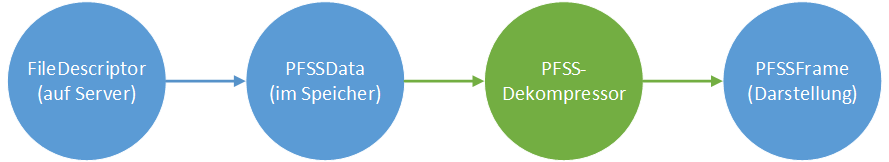
\includegraphics[width=0.6\textwidth,height=6cm,keepaspectratio]{./pictures/implementation/dataflow.png}
	\caption{Zustandsdiagramm der Feldliniendaten}
	\label{implementation:architektur:datenfluss}
\end{figure}
Die Daten der Feldlinien durchlaufen im JHelioviewer vier Zustände, welche durch vier Klassen abgebildet wurde. Die Klassen sowie die Zustandswechsel sind im Diagramm der Abbildung \ref{implementation:architektur:datenfluss} dargestellt. Die Klasse ''FileDescriptor´´ repräsentiert eine Simulation von Feldlinien auf dem Server. In diesem Zustand sind die Daten bereit für das Herunterladen. Die folgende Klasse ''PFSSData´´ symbolisiert Feldlinien, welche in den lokalen Arbeitsspeicher geladen wurden. In diesem Zustand sind die Daten noch komprimiert und nicht bereit für eine Visualisierung. Für das Herunterladen ist ebenfalls die ''PFSSData´´ Klasse zuständig. ''PFSSDekompressor´´ ist ein Zwischenzustand und stellt den Wechsel von komprimierten zu unkomprimierten Daten dar. Da der Zustandswechsel aufwändig ist, wird es durch eine eigene Klasse abgebildet. Die letzte Klasse ''PFSSFrame´´ repräsentiert die dekomprimierten Feldlinien. In diesem Zustand sind die Daten bereit für die Darstellung. Die Darstellung wird ebenfalls von der ''PFSSFrame´´ Klasse übernommen.

\subsubsection{Mehrstufiges Vorladen und Caching}
Um den Flaschenhals herunterladen und Dekomprimieren zu umgehen, wird ein mehrstufiges Read-Ahead und Caching eingeführt. Es soll ein Vorladen und Caching für die unkomprimierten ''PFSSFrame´´ Feldllinien und eines für die ''PFSSData´´ Objekte implementiert werden. Die Implementation ist im Diagramm der Abbildung \ref{implementation:architektur:caching} dargestellt.
\begin{figure}[!htbp]
	\center
	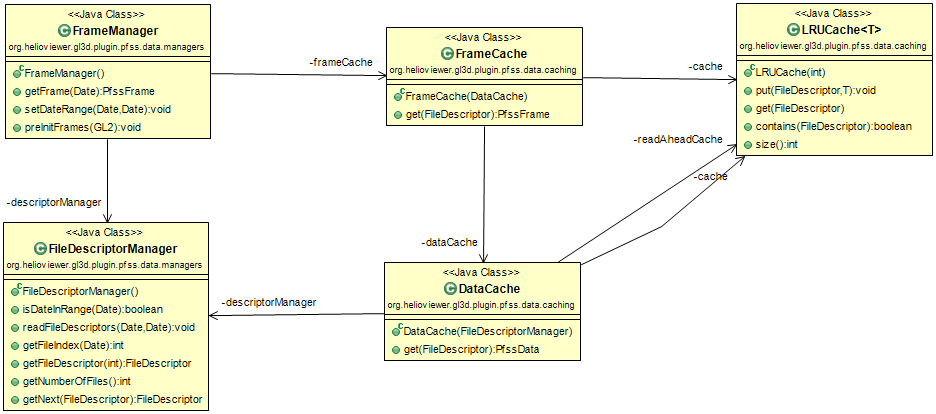
\includegraphics[width=0.9\textwidth,height=8cm,keepaspectratio]{./pictures/implementation/architectureCache.png}
	\caption{Diagramm der Implementation vom Vorladen und Caching}
	\label{implementation:architektur:caching}
\end{figure}
Der FileDescriptorManager sucht die Feldlinien auf dem Server und stellt die FileDescriptors zur Verfügung. Der Manager weiss ebenfalls, in welcher Reihenfolge die FileDescriptors zu liegen kommen.\\
Die Klasse ''Framemanager´´ ist die Facade der Vorladens- und Caching- Implementation. Sie abstrahiert das Zusammenspiel der verschiedenen Caches und den verschiedenen Zustände der Feldliniendaten, indem eine vereinfachte Schnittstelle angeboten wird. Für das Vorladen von PFSSFrame Objekte wurde wegen dem Prinzip von Low-Coupling ebenfalls im FrameManager umgesetzt. Die ''PFSSFrame´´ Objekte müssen jeweils Speicher auf der Grafikkarte alloziieren und abräumen. Die FrameManager Klasse muss genau wissen, wann ein PFSSFrame Objekt neu geladen oder nicht mehr gebraucht wird. Die Klasse FrameCache nur noch zuständig, PFSSFrame Objekte zwischenzuspeichern, welche keine Ressourcen der Grafikkarte alloziiert haben. Es ist auch eine Architektur denkbar, inder der FrameCache das Vorladen und das Abräumen des Grafikkartenspeichers übernimmt. Der Speicherplatz der Grafikkarte würde aber die Grösse des FrameCaches beschränken.\\
Das Vorladen und Caching der PFSSData Objekten wird von der Klasse DataCache übernommen. Die PFSSData Objekte alloziieren nur Arbeitsspeicher, die vom Garbage-Collector aufgeräumt werden können. Das Vorladen ist deshalb simpler und wird direkt im DataCache implementiert durch eine weitere Instanz des LRUCaches. Der eigentliche Cache beinhaltet alle PFSSData Objekte, welche gebraucht wurden und der readAheadCache alle, welche noch gebraucht werden können.\\
[\baselineskip] 
In dieser Arbeit wurde ein Least-Recently-Used (LRU) Cache Algorithmus verwendet. Wenn der Cache voll ist, löscht der Algorithmus das längste nicht verwendete Objekt. Da der JHelioviewer im allgemeinen Fall sequenzell nach den Datenobjekten abfragt, kann der LRU Cache mit einer First-in-First-out Queue implementiert werden. Das Objet, welches am längsten nicht mehr gebraucht wurde, ist das Letzte in der Queue. Ein LRU-Cache funktioniert in diesem Anwendungsfall optimal, wenn die Anzahl Objekte grösser ist, als der Cache. In einem Spezialfall ist der LRU-Algorithmus nicht optimal. Wenn der JHelioviewer zur letzten Simulation der Feldlinien angekommen ist, wird an Wrap-around durchgeführt und wieder die erste Simulation verlangt. Wenn der Cache $n-1$ von $n$ Simulation abspeichern kann, so löscht der LRU-Algorithmus immer die Simulation, welches als übernächstes abgefragt wird. Das führt dazu, dass gleich viele Cache-Misses geschehen, als wenn der Cache wesentlich kleiner währe.

\subsubsection{Asynchrone Aufrufe mittels Executor Services}
Im Diagramm der Abbildung \ref{implementation:architektur:caching} zu sehen ist, wird das Erstellen von PFSSData und PFSSFrame Objekten jeweils von zwei Klassen übernommen werden, den Creators. Sie sind zuständig für das asynchrone Herunterladen und Dekomprimieren der Feldliniendaten. Die asynchrone Ausführung ist mit dem Java Executor Service umgesetzt. Der Executor Service verwaltet und begrenzt die Anzahl an Threads welche die Aufrufe bearbeiten, sodass auch bei hoher Auslastung ein möglichst hoher Durchsatz erreicht wird. Im Ist-Zustand wurden alle asynchrone Aufrufe jeweils in einem eigenen Thread ausgeführt. Bei hoher Auslastung steigt der Verwaltungsaufwand der Threads und bremst das System.\\